\section{Evaluation}
\label{sec:eval}

% Generated by experiments/report.py from experiments/results; do not edit.
\newcommand{\EOneMeasuredA}{0.04}
\newcommand{\EOneModelA}{0.08}
\newcommand{\EOneClearA}{0.17}
\newcommand{\EOneMeasuredB}{0.15}
\newcommand{\EOneModelB}{0.23}
\newcommand{\EOneClearB}{0.20}
\newcommand{\EOneMeasuredC}{0.32}
\newcommand{\EOneModelC}{0.45}
\newcommand{\EOneClearC}{0.22}
\newcommand{\EOneMeasuredD}{0.56}
\newcommand{\EOneModelD}{0.73}
\newcommand{\EOneClearD}{0.23}
\newcommand{\EOneStdMax}{0.012}
\newcommand{\EOneClearMin}{0.173}
\newcommand{\EOneReactMin}{0.02}
\newcommand{\EOneReactMax}{0.15}
\newcommand{\EOneRatioMax}{0.79}
\newcommand{\EOneRatioMin}{0.41}
\newcommand{\EOneZeroMeasuredA}{0.06}
\newcommand{\EOneZeroModelA}{0.08}
\newcommand{\EOneZeroClearA}{0.16}
\newcommand{\EOneZeroMeasuredB}{0.20}
\newcommand{\EOneZeroModelB}{0.23}
\newcommand{\EOneZeroClearB}{0.16}
\newcommand{\EOneZeroMeasuredC}{0.40}
\newcommand{\EOneZeroModelC}{0.45}
\newcommand{\EOneZeroClearC}{0.16}
\newcommand{\EOneZeroMeasuredD}{0.68}
\newcommand{\EOneZeroModelD}{0.73}
\newcommand{\EOneZeroClearD}{0.16}
\newcommand{\EOneZeroStdMax}{0.025}
\newcommand{\EOneZeroClearMin}{0.162}
\newcommand{\EOneZeroReactMin}{0.02}
\newcommand{\EOneZeroReactMax}{0.18}
\newcommand{\EOneZeroRatioMax}{0.97}
\newcommand{\EOneZeroRatioMin}{0.51}
\newcommand{\EOneHumanSpeed}{0.5}
\newcommand{\EOneRuns}{160}
\newcommand{\EOneCollisions}{0}
\newcommand{\ETwoRuns}{240}
\newcommand{\ETwoBlindZeroMax}{0.13}
\newcommand{\ETwoBlindDistanceMax}{0.28}
\newcommand{\ETwoSilentZeroMax}{0.55}
\newcommand{\ETwoCreepMax}{0.15}
\newcommand{\EThreeHardReplaceInliersRejected}{62}
\newcommand{\EThreeHardReplaceInliersAccepted}{38}
\newcommand{\EThreeHardReplaceInliers}{3453}
\newcommand{\EThreeHardReplaceOutliersRejected}{94}
\newcommand{\EThreeHardReplaceOutliersAccepted}{6}
\newcommand{\EThreeHardReplaceOutliers}{172}
\newcommand{\EThreeHardReplaceWorstMax}{1.93}
\newcommand{\EThreeEkfTagsInliersRejected}{3}
\newcommand{\EThreeEkfTagsInliersAccepted}{97}
\newcommand{\EThreeEkfTagsInliers}{2763}
\newcommand{\EThreeEkfTagsOutliersRejected}{79}
\newcommand{\EThreeEkfTagsOutliersAccepted}{21}
\newcommand{\EThreeEkfTagsOutliers}{125}
\newcommand{\EThreeEkfTagsWorstMax}{0.31}
\newcommand{\EThreeEkfTagsScanInliersRejected}{4}
\newcommand{\EThreeEkfTagsScanInliersAccepted}{96}
\newcommand{\EThreeEkfTagsScanInliers}{2763}
\newcommand{\EThreeEkfTagsScanOutliersRejected}{78}
\newcommand{\EThreeEkfTagsScanOutliersAccepted}{22}
\newcommand{\EThreeEkfTagsScanOutliers}{125}
\newcommand{\EThreeEkfTagsScanWorstMax}{0.12}
\newcommand{\EThreeScanRejected}{0.0}
\newcommand{\EThreeDistance}{86}
\newcommand{\EThreeRuns}{20}
\newcommand{\EFourCollisions}{0}
\newcommand{\EFourRuns}{120}
\newcommand{\EFiveNoneDone}{20}
\newcommand{\EFiveNoneTime}{24.5}
\newcommand{\EFiveNoneBacked}{0.01}
\newcommand{\EFiveNoneBlocked}{0.0}
\newcommand{\EFiveFreeDone}{20}
\newcommand{\EFiveFreeTime}{41.2}
\newcommand{\EFiveFreeBacked}{1.00}
\newcommand{\EFiveFreeBlocked}{0.0}
\newcommand{\EFivePersonDone}{20}
\newcommand{\EFivePersonTime}{35.4}
\newcommand{\EFivePersonBacked}{0.49}
\newcommand{\EFivePersonBlocked}{0.0}
\newcommand{\EFivePersonBackedMin}{0.04}
\newcommand{\EFivePersonBackedMax}{0.99}
\newcommand{\EFivePersonClearMin}{0.38}
\newcommand{\EFivePersonHeld}{0}
\newcommand{\EFiveWallClearMin}{0.41}
\newcommand{\EFiveCollisions}{0}
\newcommand{\EFiveRuns}{60}
\newcommand{\EFiveSeeds}{20}


\textbf{Simulation protocol.} E1--E4 close the loop over the pure cores at the node rates:
the simulator core moves an omnidirectional body with the acceleration limits of the profile
and detects collisions; its LiDAR follows the Mid-360 (vertical field of view from $-7^\circ$ to
$52^\circ$ at the mount height, range limits, noise); odometry drifts as $\T{odom}{base}
\leftarrow \T{odom}{base} \exp(\vect{\xi})$ with $\vect{\xi} \sim \mathcal{N}(\vect{0},
\boldsymbol{\Sigma}\,\Delta s)$ plus a yaw bias and a scale error; stamps lag by 50~ms (LiDAR)
and commands by 20~ms. Perception's sector pipeline and watchdog run at 10~Hz, the follower
with the bringup's reactive policy (VFH) at 20~Hz, and every command passes the mux's arbiter
and gate, in 10~ms ticks whose task phases are drawn from the seed. All parameters are the
package defaults with the default profile ($a = 0.6$~m/s$^2$, $\tr = 0.25$~s, field margin
$m = 0.15$~m); localization is the true pose except in E3, and the health scale and the
planner's replanning are not in the loop. Each condition runs seeds 1--20; tables give mean
$\pm$ standard deviation over the 20 runs unless stated. The scripts, worlds and raw results
are in \texttt{experiments/} of the hub; one command reruns them and regenerates the tables.

\textbf{E1: stopping distance.} The robot cruises at $v$ in AUTO (a command stream at 20~Hz)
when a person (radius 0.25~m) appears on its axis $D(v) + m$ ahead of the front edge, the
nearest appearance from which \eqref{eq:braking} still promises a stop with the margin.
Table~\ref{tab:stop} gives the distance from the first safety scan that shows the person to
standstill and the smallest clearance over all runs. The robot always stopped within $D(v)$
(at most \EOneRatioMax\,$D(v)$) and never closer than \EOneClearMin~m, with no collision in
\EOneRuns{} runs; the body started braking \EOneReactMin--\EOneReactMax~s after the person
appeared, inside $\tr$. The field spends almost the whole room because it lowers the speed
along $v^*(d)$ instead of braking at once; the margin holds because the simulated body brakes
at exactly $a$, which a real robot must be shown to reach.

\begin{table}[t]
  \centering
  \caption{E1: braking model $D(v)$, measured stopping distance (mean $\pm$ std) and smallest
    clearance (all 20 runs)}
  \label{tab:stop}
  % Generated by experiments/report.py from experiments/results; do not edit.
\begin{tabular}{@{}rrrrr@{}}
  \toprule
  $v_h$ (m/s) & $v$ (m/s) & $D(v)$ (m) & measured (m) & clearance (m) \\
  \midrule
    0.5 & 0.2 & 0.08 & 0.039 $\pm$ 0.003 & 0.173 \\
    0.5 & 0.4 & 0.23 & 0.145 $\pm$ 0.006 & 0.196 \\
    0.5 & 0.6 & 0.45 & 0.317 $\pm$ 0.009 & 0.219 \\
    0.5 & 0.8 & 0.73 & 0.558 $\pm$ 0.012 & 0.234 \\
    0.0 & 0.2 & 0.08 & 0.057 $\pm$ 0.007 & 0.163 \\
    0.0 & 0.4 & 0.23 & 0.196 $\pm$ 0.012 & 0.162 \\
    0.0 & 0.6 & 0.45 & 0.399 $\pm$ 0.018 & 0.163 \\
    0.0 & 0.8 & 0.73 & 0.679 $\pm$ 0.025 & 0.162 \\
  \bottomrule
\end{tabular}

\end{table}

\textbf{E2: blind LiDAR.} The robot drives at 0.5~m/s when the LiDAR fails for 4~s: silent (no
cloud), empty (clouds without points) or sparse (50 points, below the blindness threshold of
100). Table~\ref{tab:blind} gives, in AUTO, the time $t_0$ from the failure to the first zero
command and the distance $d$ to standstill, and in REMOTE the speed of the fastest body point
during the failure, against v0.1, re-implemented as a baseline (a blind cloud gave an all-zero
scan, which the field skipped as free; no perception watchdog; field off in REMOTE). v0.2
stops an empty or sparse scan within one scan period and a silent sensor at the 0.5~s
watchdog, and caps REMOTE at the creep speed; v0.1 drove on at full speed whenever clouds kept
arriving and in REMOTE.

\begin{table}[t]
  \centering
  \caption{E2: blind LiDAR in AUTO (time to zero command, distance to standstill) and REMOTE
    (largest settled creep speed of the fastest body point), 20 runs each}
  \label{tab:blind}
  % Generated by experiments/report.py from experiments/results; do not edit.
\begin{tabular}{@{}llrrr@{}}
  \toprule
  LiDAR & stack & $t_0$ (s) & $d$ (m) & creep (m/s) \\
  \midrule
    silent & v0.2 & 0.44 $\pm$ 0.04 & 0.43 $\pm$ 0.02 & 0.15 \\
    silent & v0.1 & 0.49 $\pm$ 0.04 & 0.46 $\pm$ 0.02 & 0.50 \\
    empty & v0.2 & 0.08 $\pm$ 0.03 & 0.25 $\pm$ 0.02 & 0.15 \\
    empty & v0.1 & never & $\ge$2.0 & 0.50 \\
    sparse & v0.2 & 0.08 $\pm$ 0.03 & 0.25 $\pm$ 0.02 & 0.15 \\
    sparse & v0.1 & never & $\ge$2.0 & 0.50 \\
  \bottomrule
\end{tabular}

\end{table}

\textbf{E3: localization.} The follower drives three laps (\EThreeDistance~m) of the mall
route of the simulator with the odometry drift of its drift scenario (1~cm$/\sqrt{\mathrm{m}}$,
$0.3^\circ/\sqrt{\mathrm{m}}$, 1\,\% scale, $0.1^\circ$/m yaw bias); four tags hang at the
corridor ends. A forward camera detects them at 5~Hz up to 5~m with the noise the tag source
assumes, and 5\,\% of the detections are outliers (heading 5--25$^\circ$, position
0.1--0.4~m off, like the pose ambiguity of a small tag). The three estimators get the same
odometry, detections and scans; scan matching runs at 1~Hz on the site map the simulator draws.
Table~\ref{tab:loc} and Fig.~\ref{fig:loc} show the errors against the true pose. Hard
replacement rejected \EThreeHardReplaceInliersRejected\,\% of the good detections, because
its 0.5~m threshold compares the change of \frm{map}$\to$\frm{odom}, which grows with the
distance from the odometry origin, and still accepted \EThreeHardReplaceOutliersAccepted\,\% of the outliers; the
chi-square gate rejected \EThreeEkfTagsOutliersRejected\,\% of the outliers and
\EThreeEkfTagsInliersRejected\,\% of the good detections, and no scan match
(\EThreeScanRejected\,\% rejected).

\begin{table}[t]
  \centering
  \caption{E3: localization error under seeded drift: RMSE of position (ATE), largest position
    error and RMSE of heading per run}
  \label{tab:loc}
  % Generated by experiments/report.py from experiments/results; do not edit.
\begin{tabular}{@{}lrrr@{}}
  \toprule
  Method & ATE (m) & max (m) & yaw (°) \\
  \midrule
    Hard replace (v0.1) & 0.430 $\pm$ 0.244 & 1.15 $\pm$ 0.42 & 3.27 $\pm$ 1.63 \\
    EKF, tags & 0.074 $\pm$ 0.009 & 0.21 $\pm$ 0.03 & 0.86 $\pm$ 0.21 \\
    EKF, tags + scan match & 0.028 $\pm$ 0.002 & 0.08 $\pm$ 0.01 & 0.46 $\pm$ 0.08 \\
  \bottomrule
\end{tabular}

\end{table}

\begin{figure}[t]
  \centering
  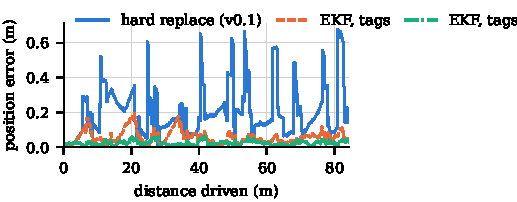
\includegraphics[width=\columnwidth]{figures/e3_error}
  \caption{E3, seed 1: position error over the distance driven.}
  \label{fig:loc}
\end{figure}

\textbf{E4: path shift.} The follower drives 20~m along the centre of a 3~m corridor: a person
stands on the route (\emph{on}) or both standing people stand 0.6--0.9~m beside it on opposite
sides (\emph{beside}), a third walks the same way at 0.2~m/s and a fourth crosses at 0.6~m/s
3~m ahead of the robot; people do not give way. Table~\ref{tab:shift} gives the completed runs,
their time, the stops before the goal, the smallest clearance to a person and the largest
distance from the route. \todo{E4 text}

\begin{table}[t]
  \centering
  \caption{E4: corridor with people (20 runs each): completed, time and stops (completed runs,
    mean $\pm$ std), smallest clearance and largest offset (all runs)}
  \label{tab:shift}
  \setlength{\tabcolsep}{3pt}
  % Generated by experiments/report.py from experiments/results; do not edit.
\begin{tabular}{@{}llrrrrr@{}}
  \toprule
  people & avoidance & done & time (s) & stops & clear. (m) & offset (m) \\
  \midrule
    on & path shift & 17/20 & 71.6 $\pm$ 1.7 & 1.2 $\pm$ 0.5 & 0.22 & 0.80 \\
    on & reactive & 0/20 & -- & -- & 0.35 & 0.01 \\
    on & none & 0/20 & -- & -- & 0.32 & 0.00 \\
    beside & path shift & 20/20 & 71.4 $\pm$ 1.7 & 1.2 $\pm$ 0.6 & contact & 0.79 \\
    beside & reactive & 13/20 & 70.9 $\pm$ 1.6 & 8.2 $\pm$ 2.4 & 0.12 & 0.00 \\
    beside & none & 13/20 & 70.9 $\pm$ 1.7 & 7.8 $\pm$ 1.9 & 0.12 & 0.00 \\
  \bottomrule
\end{tabular}

\end{table}

\textbf{End to end.} \todo{e2e}
